%
% hmo_energiediagramm.tex
%
% (c) 2025 Prof Dr Andreas Müller
%
\documentclass[tikz]{standalone}
\usepackage{amsmath}
\usepackage{times}
\usepackage{txfonts}
\usepackage{pgfplots}
\usetikzlibrary{arrows.meta}

\begin{document}

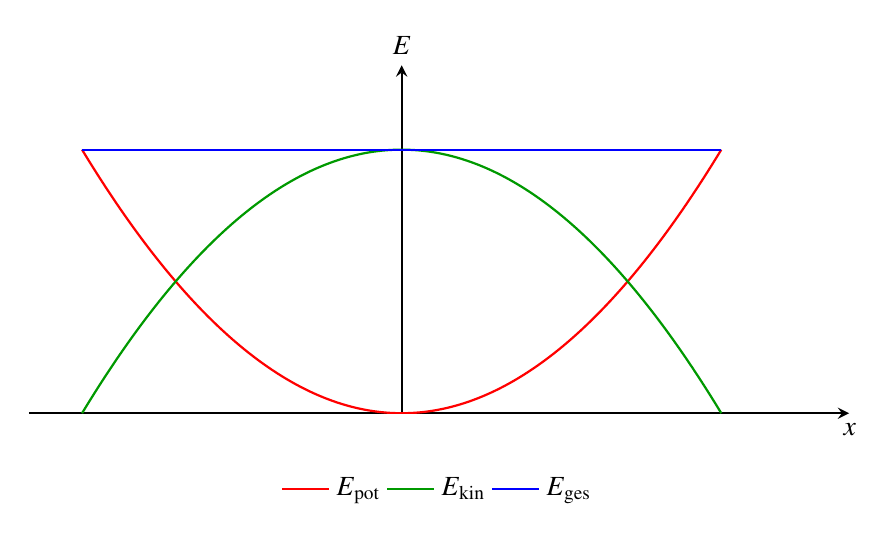
\begin{tikzpicture}
    \begin{axis}[
        axis lines=middle,
        xlabel={$x$},
        ylabel={$E$},
        enlargelimits=upper,
        axis line style={thick},
        xmin=-3.5, xmax=3.5,
        ymin=0, ymax=1.2,
        xtick=\empty,
        ytick=\empty,
        width=12cm,
        height=6cm,
        samples=200,
        domain=-3:3,
        thick,
        every axis x label/.style={at={(ticklabel* cs:1)}, anchor=north},
        every axis y label/.style={at={(ticklabel* cs:1)}, anchor=south},
        legend style={draw=none, at={(0.5,-0.15)}, anchor=north, legend columns=3},
    ]
    
    % Epot: rote Parabel, Scheitel bei x=0
    \addplot[red, thick, domain=-3:3] {x^2/9};
    \addlegendentry{$E_{\text{pot}}$}
    
    % Ekin: grüne umgedrehte Parabel, Scheitel bei x=0
    \addplot[green!60!black, thick, domain=-3:3] {1 - x^2/9};
    \addlegendentry{$E_{\text{kin}}$}
    
    % Eges: konstante blaue Linie
    \addplot[blue, thick, domain=-3:3] {1};
    \addlegendentry{$E_{\text{ges}}$}
    
    \end{axis}
\end{tikzpicture}

\end{document}
